\documentclass[11pt,a4paper]{article}
\usepackage[a4paper,margin=2.1cm]{geometry}
\usepackage[T1]{fontenc}
\usepackage{lmodern,microtype}
\usepackage{amsmath,amssymb}
\usepackage{graphicx,booktabs,caption,subcaption}
\usepackage[dvipsnames]{xcolor}
\usepackage[colorlinks=true,linkcolor=NavyBlue,urlcolor=NavyBlue,citecolor=NavyBlue]{hyperref}
\usepackage{enumitem}
\setlist{nosep,leftmargin=1.2em}
\captionsetup{font=small,labelfont=bf}
\graphicspath{{../results/}}
\setlength{\parskip}{0.35em}
\setlength{\parindent}{0pt}

\title{\vspace{-1.2cm}\textbf{Monte Carlo Pricing of Vanilla and Exotic Options}\\[0.2em]
\large Summary of results}
\author{Luca Dennert\\\small Università Bocconi -- MSc in Finance\\
\small\url{https://github.com/LucaDennert/mc-option-pricing}}
\date{November 2026}

\begin{document}
\maketitle
\vspace{-0.6cm}

\begin{abstract}
\noindent This note summarises the numerical results of \texttt{mcpricer}, a Monte Carlo library
for single-asset equity derivatives under Black--Scholes, Heston and Merton dynamics. Every
estimator is validated against a closed-form or semi-analytic benchmark. Four findings stand out:
(i)~randomised quasi-Monte Carlo converges at close to $O(N^{-1})$, about $400\times$ more accurate
than plain Monte Carlo at $1.3\times10^5$ paths; (ii)~for arithmetic Asians, combining Sobol
points, a Brownian bridge and a geometric-Asian control variate cuts the variance by a factor of
$\sim\!2\times10^4$; (iii)~discretely monitored barriers carry a large bias that the Brownian-bridge
correction removes even on a coarse grid, and Andersen's QE scheme removes the Heston
discretisation bias with $\sim\!8$ steps per year against $>100$ for Euler; (iv)~with Heston and
Black--Scholes matched on the at-the-money price, exotic prices differ by up to 35\% of the
Black--Scholes value for digitals and by a factor of $3.5$ for knock-in puts.
\end{abstract}

\section{Setup}
\textbf{Models.} Black--Scholes (exact log-normal stepping); Heston with Andersen's (2008)
quadratic-exponential (QE) scheme, compared with full-truncation Euler; Merton jump-diffusion
(exact, Poisson counts by inverse CDF). \textbf{Products.} European, digital, arithmetic and
geometric Asian, the eight single barriers, fixed and floating lookbacks, and a Phoenix
autocallable with memory coupon and European knock-in. \textbf{Variance reduction.} Antithetic
variates, control variates with optimal $\beta$, scrambled Sobol sequences with a Brownian-bridge
construction. Standard errors use the antithetic pair as the i.i.d.\ unit, and 16 independent
scramblings for RQMC. \textbf{Benchmarks.} Black--Scholes, Reiner--Rubinstein barriers,
Kemna--Vorst geometric Asian (arbitrary fixings), Goldman--Sosin--Gatto lookback, Merton series
and the Heston ``little trap'' characteristic function. The test-suite (47 tests) checks every
Monte Carlo price against these within a few standard errors.

Unless stated otherwise: $S_0=K=100$, $T=1$, $r=3\%$, $q=1\%$, $\sigma=20\%$.

\section{Convergence and variance reduction}
\begin{figure}[h]
\centering
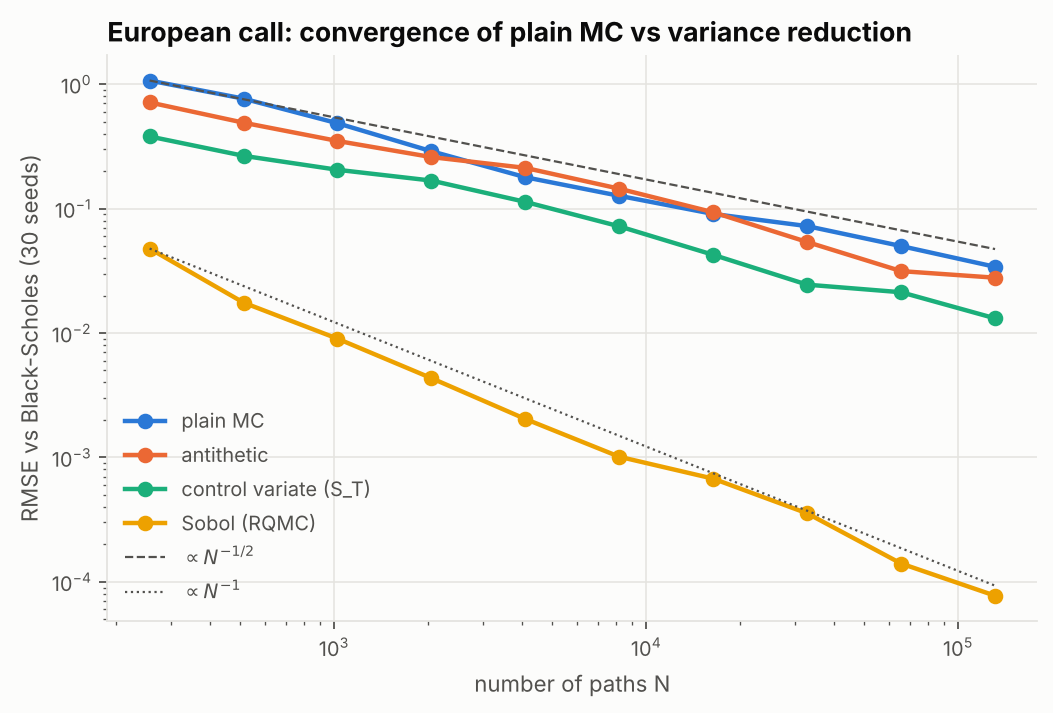
\includegraphics[width=0.66\textwidth]{convergence_european.png}
\caption{RMSE of the European call price against Black--Scholes over 30 independent seeds.}
\label{fig:conv}
\end{figure}

Pseudo-random estimators converge at the canonical $O(N^{-1/2})$ rate (Figure~\ref{fig:conv});
antithetics and a control variate on $S_T$ shift the line down without changing its slope.
Scrambled Sobol points converge at close to $O(N^{-1})$: at $N=131{,}072$ the RMSE is
$7.7\times10^{-5}$ against $3.4\times10^{-2}$ for plain Monte Carlo.

\begin{table}[h]
\centering\small
\begin{tabular}{lrrr}
\toprule
Method & Price & Std.\ error & Variance reduction \\
\midrule
Plain Monte Carlo & 5.3135 & $3.13\times10^{-2}$ & 1 \\
Antithetic & 5.3327 & $2.35\times10^{-2}$ & 2 \\
Geometric-Asian control variate & 5.3256 & $8.41\times10^{-4}$ & 1{,}389 \\
Sobol + Brownian bridge (RQMC) & 5.3245 & $7.54\times10^{-4}$ & 1{,}726 \\
\textbf{Sobol + Brownian bridge + control variate} & \textbf{5.3247} & $\mathbf{2.04\times10^{-4}}$ & \textbf{23{,}585} \\
\bottomrule
\end{tabular}
\caption{Arithmetic Asian call, 12 monthly fixings, $N=65{,}536$ paths. Variance reduction is
relative to plain Monte Carlo; CPU time is essentially unchanged across methods.}
\label{tab:asian}
\end{table}

For path-dependent payoffs the gains compound (Table~\ref{tab:asian}). The geometric Asian has an
exact price for any set of fixing dates and is almost perfectly correlated with the arithmetic
average, so it is a near-ideal control variate; the Brownian bridge places the variance of the
terminal value in the first, best-distributed Sobol dimensions.

\section{Discretisation: barriers and Heston}
\begin{figure}[h]
\centering
\begin{subfigure}{0.49\textwidth}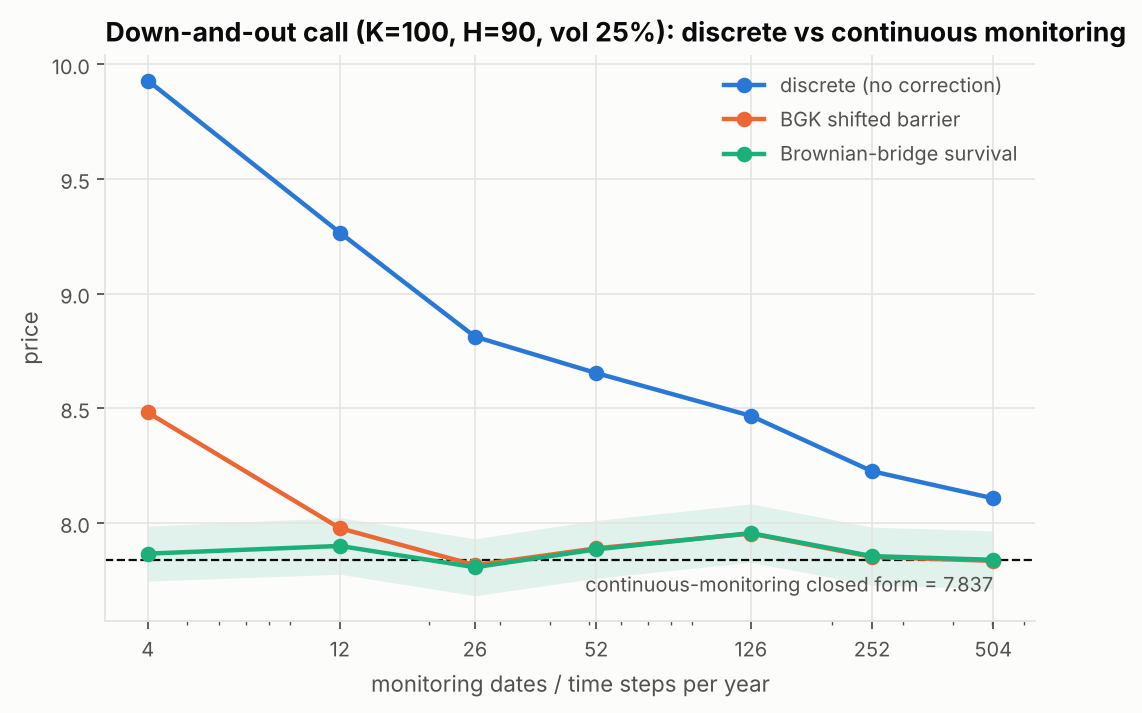
\includegraphics[width=\linewidth]{barrier_monitoring.png}
\caption{Down-and-out call, $H=90$, $\sigma=25\%$.}\end{subfigure}\hfill
\begin{subfigure}{0.49\textwidth}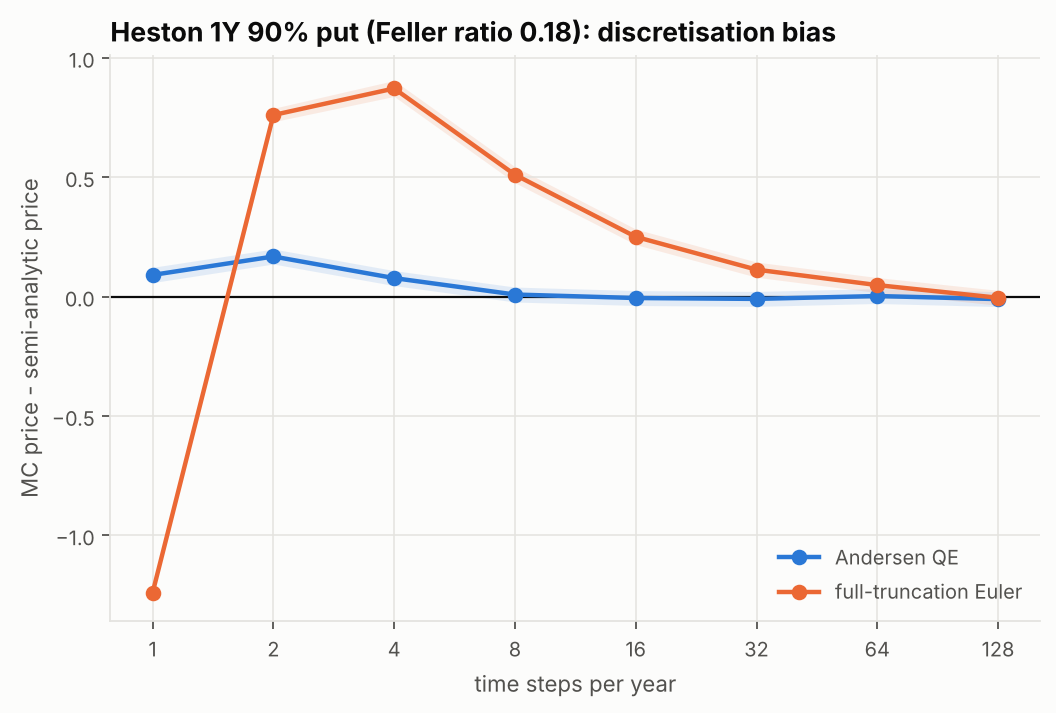
\includegraphics[width=\linewidth]{heston_schemes.png}
\caption{Heston 1Y 90\% put, Feller ratio 0.18.}\end{subfigure}
\caption{Bias against the continuous-time benchmark as a function of the time grid.}
\label{fig:disc}
\end{figure}

\textbf{Barriers.} Checking the barrier only on the grid misses crossings between dates: with
monthly monitoring the knock-out call is overpriced by 18\% (9.27 against 7.84). The
Broadie--Glasserman--Kou shift $H\to He^{\pm0.5826\,\sigma\sqrt{\Delta t}}$ removes most of the bias
from about 12 dates, while the exact Brownian-bridge survival probability between grid points,
$1-\exp\!\big(-2\ln(S_i/H)\ln(S_{i+1}/H)/(\sigma^2\Delta t)\big)$, is unbiased even with four steps
(Figure~\ref{fig:disc}a).

\textbf{Heston.} With index-like parameters ($\kappa=1.8$, $\theta=0.045$, $\xi=0.95$,
$\rho=-0.75$) the Feller condition fails and the variance spends long periods near zero.
Full-truncation Euler needs over 100 steps per year to bring the bias inside the confidence band;
the QE scheme, which matches the first two conditional moments of the non-central $\chi^2$
transition, is unbiased from about 8 steps per year (Figure~\ref{fig:disc}b).

\section{Calibration and model risk on exotics}
Heston is calibrated by vega-weighted least squares on the out-of-the-money surface, using
Gil-Pelaez inversion of the characteristic function. The OptionMetrics pipeline builds this
surface from IvyDB quotes, with forwards and dividend yields implied from put-call parity.
\emph{The figures in this note use a synthetic SPX-like surface (Heston with bid--ask noise),
so the calibration step is a correctness check: the true parameters are recovered to within
1\% with an implied-vol RMSE of 0.03 vol points (Figure~\ref{fig:fit}). The same scripts run
unchanged on OptionMetrics data.}

\begin{figure}[h]
\centering
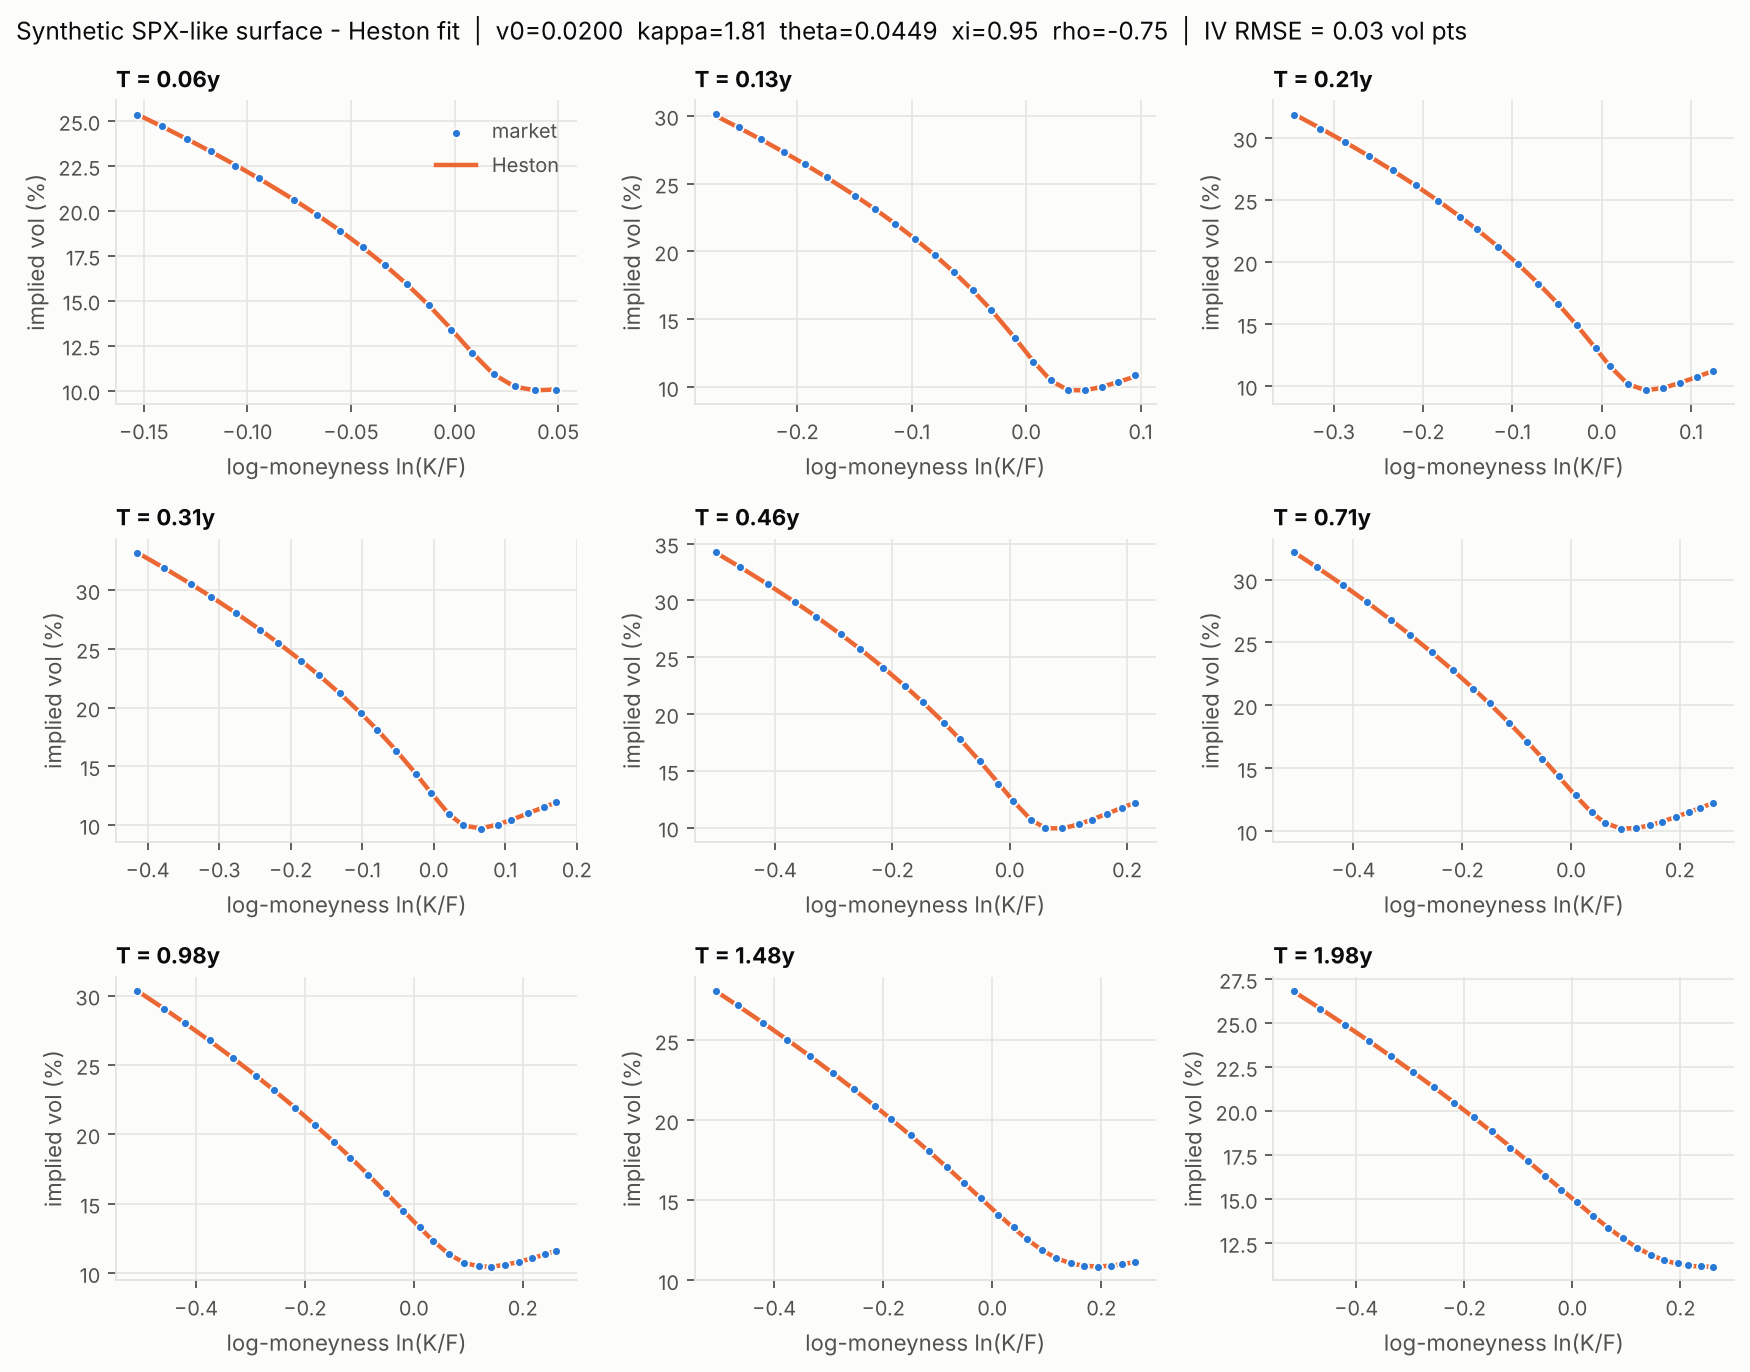
\includegraphics[width=\textwidth]{heston_fit_synthetic_spx_surface.png}
\caption{Heston fit across nine maturities (synthetic SPX-like surface).}
\label{fig:fit}
\end{figure}

\begin{table}[h]
\centering\small
\begin{tabular}{lrrr}
\toprule
Product (prices in \% of spot) & Black--Scholes & Heston & Difference \\
\midrule
ATM call 1Y & 7.47 & 7.45 & $-0.02$ \\
Digital call 105\% 1Y (pays 100) & 40.56 & 54.84 & $+14.27$ \\
Down-and-out call K100 H80 1Y & 7.46 & 7.22 & $-0.24$ \\
Down-and-in put K100 H75 1Y & 0.94 & 3.34 & $+2.40$ \\
Up-and-out call K100 H120 1Y & 2.18 & 5.59 & $+3.41$ \\
Asian call (12 fixings) 1Y & 4.43 & 4.24 & $-0.19$ \\
Floating lookback call 1Y & 12.22 & 13.72 & $+1.50$ \\
Phoenix autocallable 3Y (2\% quarterly coupon, KI 60\%) & 101.69 & 100.27 & $-1.43$ \\
\bottomrule
\end{tabular}
\caption{Black--Scholes uses the Heston-implied ATM-spot volatility of each maturity (15.0\% at
1Y, 17.6\% at 3Y), so the two models agree on the ATM call (difference within one standard error,
0.018). Daily monitoring; 131k antithetic paths; Heston standard errors $\le 0.12$.}
\label{tab:exotics}
\end{table}

Table~\ref{tab:exotics} isolates the price of the smile. Under skew, a digital call is minus the
strike-derivative of the call price, $D = D_{BS} - \text{Vega}\cdot\partial\sigma/\partial K$, so
negative skew makes it 35\% more expensive. The knock-in put sits where implied volatility is
highest, and a flat-volatility model undervalues it by a factor of 3.5. Because the holder of a
Phoenix certificate is short that put, flat-volatility pricing overstates the certificate's fair
value by about 1.4 points of notional. The up-and-out call is worth more under Heston because
upside implied volatility is low ($\approx\!10\%$), so the barrier is touched less often.

\section{Greeks}
\begin{table}[h]
\centering\small
\begin{tabular}{lrrl}
\toprule
Greek & Closed form & Bump \& revalue (CRN) & Single-run estimator \\
\midrule
Call delta & 0.5735 & 0.5735 & pathwise $0.5747\pm0.0026$ \\
Call gamma & 0.0194 & 0.0193 & -- \\
Call vega & 38.715 & 38.780 & -- \\
Digital delta & 0.0194 & 0.0196 & likelihood ratio $0.0193\pm0.0001$ \\
\bottomrule
\end{tabular}
\caption{ATM 1Y options, 131k antithetic paths, common random numbers for the bumps.}
\label{tab:greeks}
\end{table}

Bumping with common random numbers recovers all Greeks to three significant digits
(Table~\ref{tab:greeks}). For the digital, the pathwise estimator is zero almost surely because
the payoff is discontinuous; the likelihood-ratio estimator differentiates the density instead
and stays unbiased.

\section{Takeaways}
\begin{itemize}
\item Error bars matter as much as prices: antithetic pairs and RQMC replications give honest
standard errors.
\item Quasi-Monte Carlo with a Brownian bridge, plus an analytic control variate where one exists,
is the default choice for smooth path-dependent payoffs.
\item Discretisation bias, not sampling error, dominates for barriers and for Heston with Euler;
analytic corrections (Brownian bridge, QE) fix it at almost no cost.
\item Matching the ATM price is not enough: digitals, barriers and autocallables are priced by the
smile, so the choice of model changes their value by several points of notional.
\end{itemize}

\vspace{0.3em}
{\small\textbf{References.} Andersen (2008), \emph{J.\ Comput.\ Finance} 11(3);
Albrecher et al.\ (2007), \emph{Wilmott}; Broadie, Glasserman \& Kou (1997), \emph{Math.\ Finance} 7(4);
Glasserman (2003), \emph{Monte Carlo Methods in Financial Engineering}; Heston (1993), \emph{RFS} 6(2);
Kemna \& Vorst (1990), \emph{JBF} 14(1); Merton (1976), \emph{JFE} 3; Reiner \& Rubinstein (1991), \emph{Risk} 4(8).}

\end{document}
